\documentclass[tikz,border=4pt]{standalone}
\usepackage[T1]{fontenc}
\usepackage{newtxtext}
\usetikzlibrary{positioning,arrows.meta,fit,backgrounds,shapes.geometric,calc}

\definecolor{garnet}{HTML}{8F001A}
\definecolor{blueA}{HTML}{2B6CB0}
\definecolor{orangeA}{HTML}{D9822B}
\definecolor{greenA}{HTML}{2F855A}
\definecolor{greyA}{HTML}{F2F2F2}
\definecolor{greyB}{HTML}{D9D9D9}
\definecolor{ink}{HTML}{2D2D2C}
\definecolor{paleBlue}{HTML}{E6EFF9}
\definecolor{paleGreen}{HTML}{E7F3EC}
\definecolor{paleGarnet}{HTML}{F7E8EB}

\begin{document}
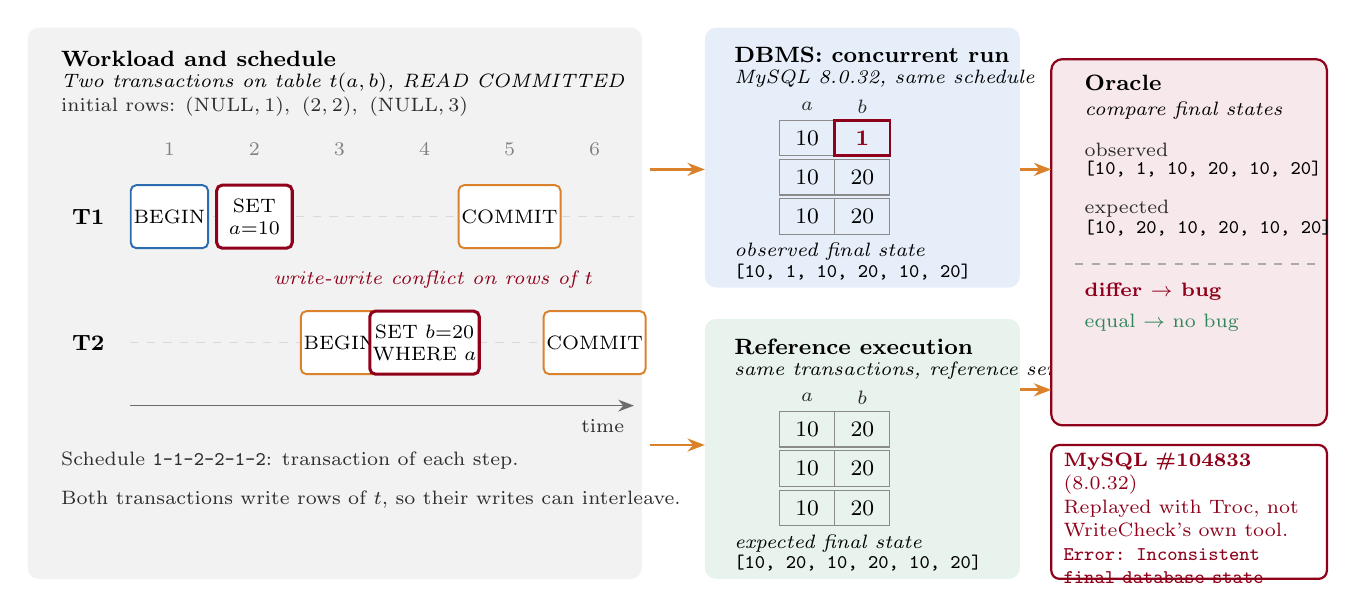
\begin{tikzpicture}[
  font=\scriptsize\color{ink},
  >={Stealth[length=2.2mm]},
  box/.style={rounded corners=2pt, fill=white, line width=0.7pt,
    minimum width=0.96cm, minimum height=0.8cm, inner sep=1pt,
    align=center, font=\scriptsize},
  cell/.style={draw=ink!55, minimum width=0.7cm, minimum height=0.45cm,
    inner sep=0pt, font=\footnotesize},
]

% ---------- Panel A: workload and schedule ----------
\fill[greyA, rounded corners=4pt] (0,0) rectangle (7.8,7.0);
\node[anchor=west, font=\footnotesize\bfseries] at (0.3,6.6) {Workload and schedule};
\node[anchor=west, font=\scriptsize\itshape] at (0.3,6.3) {Two transactions on table $t(a,b)$, READ COMMITTED};
\node[anchor=west] at (0.3,6.0) {initial rows: $(\mathrm{NULL},1),\ (2,2),\ (\mathrm{NULL},3)$};

% step columns 1..6 follow the schedule 1-1-2-2-1-2
\foreach \k/\x in {1/1.8, 2/2.88, 3/3.96, 4/5.04, 5/6.12, 6/7.2}
  \node[color=ink!60] at (\x,5.45) {\k};

\draw[dashed, greyB, line width=0.6pt] (1.3,4.6) -- (7.7,4.6);
\draw[dashed, greyB, line width=0.6pt] (1.3,3.0) -- (7.7,3.0);
\node[anchor=east, font=\footnotesize\bfseries] at (1.1,4.6) {T1};
\node[anchor=east, font=\footnotesize\bfseries] at (1.1,3.0) {T2};

\node[box, draw=blueA] at (1.8,4.6)  {BEGIN};
\node[box, draw=garnet, line width=1.1pt] at (2.88,4.6) {SET\\$a{=}10$};
\node[box, draw=orangeA] at (6.12,4.6) {COMMIT};

\node[box, draw=orangeA] at (3.96,3.0) {BEGIN};
\node[box, draw=garnet, line width=1.1pt] at (5.04,3.0) {SET $b{=}20$\\WHERE $a$};
\node[box, draw=orangeA] at (7.2,3.0) {COMMIT};

\node[font=\scriptsize\itshape, text=garnet, anchor=west] at (3.0,3.8) {write-write conflict on rows of $t$};

\draw[-{Stealth[length=2mm]}, ink!70, line width=0.6pt] (1.3,2.2) -- (7.7,2.2);
\node[anchor=north east] at (7.7,2.15) {time};

\node[anchor=west] at (0.3,1.5) {Schedule \texttt{1-1-2-2-1-2}: transaction of each step.};
\node[anchor=west] at (0.3,1.0) {Both transactions write rows of $t$, so their writes can interleave.};

% ---------- Panel B: concurrent DBMS run ----------
\fill[paleBlue, rounded corners=4pt] (8.6,3.7) rectangle (12.6,7.0);
\node[anchor=west, font=\footnotesize\bfseries] at (8.85,6.65) {DBMS: concurrent run};
\node[anchor=west, font=\scriptsize\itshape] at (8.85,6.35) {MySQL 8.0.32, same schedule};

\node at (9.9,6.0) {$a$};
\node at (10.6,6.0) {$b$};
\node[cell] at (9.9,5.6)  {10};
\node[cell, draw=garnet, line width=1pt, text=garnet, font=\footnotesize\bfseries] at (10.6,5.6) {1};
\node[cell] at (9.9,5.1)  {10};
\node[cell] at (10.6,5.1) {20};
\node[cell] at (9.9,4.6)  {10};
\node[cell] at (10.6,4.6) {20};
\node[anchor=west, font=\scriptsize\itshape] at (8.85,4.15) {observed final state};
\node[anchor=west, font=\ttfamily\scriptsize] at (8.85,3.9) {[10, 1, 10, 20, 10, 20]};

% ---------- Panel C: reference execution ----------
\fill[paleGreen, rounded corners=4pt] (8.6,0.0) rectangle (12.6,3.3);
\node[anchor=west, font=\footnotesize\bfseries] at (8.85,2.95) {Reference execution};
\node[anchor=west, font=\scriptsize\itshape] at (8.85,2.65) {same transactions, reference semantics};

\node at (9.9,2.3) {$a$};
\node at (10.6,2.3) {$b$};
\node[cell] at (9.9,1.9)  {10};
\node[cell] at (10.6,1.9) {20};
\node[cell] at (9.9,1.4)  {10};
\node[cell] at (10.6,1.4) {20};
\node[cell] at (9.9,0.9)  {10};
\node[cell] at (10.6,0.9) {20};
\node[anchor=west, font=\scriptsize\itshape] at (8.85,0.45) {expected final state};
\node[anchor=west, font=\ttfamily\scriptsize] at (8.85,0.2) {[10, 20, 10, 20, 10, 20]};

% ---------- Oracle ----------
\fill[paleGarnet, rounded corners=4pt] (13.0,1.95) rectangle (16.5,6.6);
\draw[garnet, line width=0.8pt, rounded corners=4pt] (13.0,1.95) rectangle (16.5,6.6);
\node[anchor=west, font=\footnotesize\bfseries] at (13.3,6.3) {Oracle};
\node[anchor=west, font=\scriptsize\itshape] at (13.3,5.95) {compare final states};
\node[anchor=west] at (13.3,5.45) {observed};
\node[anchor=west, font=\ttfamily\scriptsize] at (13.3,5.2) {[10, 1, 10, 20, 10, 20]};
\node[anchor=west] at (13.3,4.7) {expected};
\node[anchor=west, font=\ttfamily\scriptsize] at (13.3,4.45) {[10, 20, 10, 20, 10, 20]};
\draw[dashed, ink!40, line width=0.5pt] (13.3,4.0) -- (16.35,4.0);
\node[anchor=west, font=\scriptsize\bfseries, text=garnet] at (13.3,3.65) {differ $\rightarrow$ bug};
\node[anchor=west, font=\scriptsize, text=greenA] at (13.3,3.25) {equal $\rightarrow$ no bug};

% ---------- Garnet callout ----------
\draw[garnet, line width=0.8pt, fill=white, rounded corners=3pt] (13.0,0.0) rectangle (16.5,1.7);
\node[anchor=north west, text=garnet, text width=3.0cm, align=left, inner sep=0pt]
  at (13.15,1.6) {\textbf{MySQL \#104833} (8.0.32)\\[1pt]
  Replayed with Troc, not WriteCheck's own tool.\\[1pt]
  \texttt{Error: Inconsistent final database state}};

% ---------- Flow arrows ----------
\draw[-{Stealth[length=2.2mm]}, orangeA, line width=1pt] (7.9,5.2) -- (8.6,5.2);
\draw[-{Stealth[length=2.2mm]}, orangeA, line width=1pt] (7.9,1.7) -- (8.6,1.7);
\draw[-{Stealth[length=2.2mm]}, orangeA, line width=1pt] (12.6,5.2) -- (13.0,5.2);
\draw[-{Stealth[length=2.2mm]}, orangeA, line width=1pt] (12.6,2.4) -- (13.0,2.4);

\end{tikzpicture}
\end{document}
